\def\layersep{2.7cm}

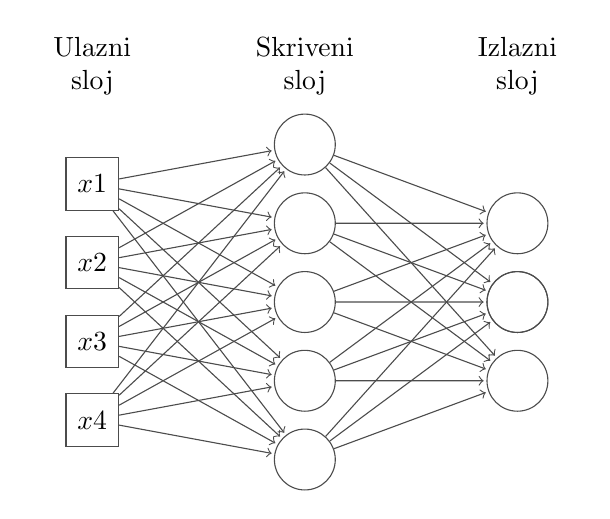
\begin{tikzpicture}[shorten >=1pt,->,draw=black!70, node distance=\layersep]
    \tikzstyle{every pin edge}=[thick,<-,shorten <=1pt]
    \tikzstyle{smallneuron}=[rectangle, draw, minimum size=19pt]
    \tikzstyle{neuron}=[draw, circle,minimum size=22pt]
    \tikzstyle{annot} = [text width=4em, text centered]

    % Draw the input layer nodes
    \foreach \name / \y in {1,...,4}
    % This is the same as writing \foreach \name / \y in {1/1,2/2,3/3,4/4}
        \node[smallneuron] (I-\name) at (0,-\y) {$x\y$};

    % Draw the hidden layer nodes
    \foreach \name / \y in {1,...,5}
        \path[yshift=0.5cm]
            node[neuron] (H-\name) at (\layersep,-\y cm) {};

    \foreach \name / \y in {1,...,3}
        \path[yshift=-0.5cm]
            node[neuron] (O-\name) at (2*\layersep,-\y cm) {};

    % Draw the output layer node
    \node[neuron, right of=H-3] (O) {};



    % Connect every node in the input layer with every node in the
    % hidden layer.
    \foreach \source in {1,...,4}
        \foreach \dest in {1,...,5}
            \path (I-\source) edge (H-\dest);

    \foreach \source in {1,...,5}
        \foreach \dest in {1,...,3}
            \path (H-\source) edge (O-\dest);

    % % Connect every node in the hidden layer with the output layer
    % \foreach \source in {1,...,5}
    %     \path (H-\source) edge (O);

    % Annotate the layers
    \node[annot,above of=H-1, node distance=1cm] (hl) {Skriveni sloj};
    \node[annot,left of=hl] {Ulazni sloj};
    \node[annot,right of=hl] {Izlazni sloj};
\end{tikzpicture}
